\section{Numerical Results}
\label{sec:results}

\subsection{Adaptive Methods}

In this subsection we show some numerical tests to validate the utility of the
adaptive approaches for the selection of the number of permutations to employ.
For this purpose, we restrict our attention to standard Monte Carlo linear
solvers.

At first we take into account the Forward Monte Carlo linear solver.
In particular, the adaptive threshold associated with formulas
(\ref{forward_adapt}) and
(\ref{adjoint_adapt}) is set to $\varepsilon_1=0.1$ and to
$\varepsilon_1=0.01$. \newline

A set of matrices associated with problems of various nature has been collected.
All the problems treated have a small number of d.o.f's to control the
massive computational cost of MC solvers on a standard laptop. All the analyzed
matrices are derived from the
discretization of other differential problems.
One of these matrices is produced by the finite volume discretization of
a thermal equation (Marshak problem), another one is a 1D diffusion reaction
problem discretized with finite differences, a
2D laplacian discretized with finite differences and an advection
diffusion
problem discretized with quadrilateral linear finite elements (the
\texttt{ifiss} package is used in this case).
For all the problems at hand a left diagonal preconditioning is applied.
Details about all these matrices are gathered in Table
\ref{table_data}.

\begin{table}[!h]
\centering
\begin{tabular}{|c|c|c|c|c|}
\hline
\textbf{Type of problem} & \textbf{d.o.f.'s} &
$\rho(H)$&Forward $\rho(\hat{H})$&Adjoint $\rho(\hat{H})$\\
\hline
1d shifted Laplacian & 50 & $0.4991$ & $0.9827$ & $0.9827$\\
\hline
2d Laplacian & 900 & $0.9949$ & $0.994$ & $0.9945$\\
\hline
ifiss & 1089 &$0.9836$ & $0.983$ & $0.983$ \\
\hline
Marshak Equation & 1600 & $0.6009$ & $0.3758$ & $ 0.3815$ \\
\hline
\end{tabular}
\caption{Properties of the matrices employed for the checks on adaptivity.}
\label{table_data}
\end{table}

For all the numerical tests results are presented both by using the Forward
and the Adjoint Monte Carlo.

As concerns the Forward method, a safety threshold for maximal number of
histories per
entry is set to $10^7$. Results are presented for
$\varepsilon_1=0.1$ and $\varepsilon_1=0.01$ in Tables \ref{tab:For_adapt} and
\ref{tab:For_adapt2} respectively. A batch size of two is used at each
adaptive check to verify the magnitude of the apparent relative standard
deviation. As expected, results are aligned with the convergence rate predicted
by the Central Limit Theorem. Indeed, decreasing of a factor of 10 the
tolerance $\varepsilon_1$, the relative error decreases of the same order,
employing in average one hundred times more histories.\newline


\begin{table}[!h]
\centering
\begin{tabular}{|c|c|c|}
\hline
\textbf{Type of problem} & \textbf{Relative Error} &\textbf{Nb. Histories}\\
\hline
1d shifted Laplacian & $0.003$ & $5,220$\\
\hline
2d Laplacian & $0.1051$ & $262,350$\\
\hline
ifiss advection diffusion & $0.022$  & $1,060,770$\\
\hline
Marshak equation & $0.0012$ & $1,456,000$\\
\hline
\end{tabular}
\caption{Forward Monte Carlo. Adaptive selection of histories.
$\varepsilon_1=0.1$}
\label{tab:For_adapt}
\end{table}

\begin{table}[!h]
\centering
\begin{tabular}{|c|c|c|}
\hline
\textbf{Type of problem} & \textbf{Relative Error} &\textbf{Nb. Histories}\\
\hline
1d shifted Laplacian & $4\cdot 10^{-4}$ & $512,094$\\
\hline
2d Laplacian & $0.0032$ & $108,551,850$\\
\hline
ifiss advection diffusion & $0.0023$  & $105,476,650$\\
\hline
Marshak equation & $5.8 \cdot 10^{-4}$ & $144,018,700$\\
\hline
\end{tabular}
\caption{Forward Monte Carlo. Adaptive selection of histories.
$\varepsilon_1=0.01$}
\label{tab:For_adapt2}
\end{table}

As regards the Adjoint Monte Carlo, at each adaptive check the number of
random walks employed is increased by ten.

A maximal number of histories equal to $10^10$ is employed as a safety
threshold.

Here below Tables \ref{tab:Adj_adapt}, \ref{tab:Adj_adapt2} and
\ref{tab:Adj_adapt3} show results
for the different test cases
considered using $\varepsilon_1=0.1$, $\varepsilon_1=0.01$ and
$\varepsilon_1=10^{-3}$ respectively.
By comparing the two tables, it is noticed that a decrease of the threshold
induces a reduction of the relative error of the same order of magnitude.
Therefore this validates
the effectiveness of the adaptive selection of histories with an error
reduction goal. The total number of histories employed increases on average by
two orders of magnitude and this aspect is in line too with what expected by
theoretical results.

\begin{table}[!h]
\centering
\begin{tabular}{|c|c|c|}
\hline
\textbf{Type of problem} & \textbf{Relative Error} &\textbf{Nb. Histories}\\
\hline
1d shifted Laplacian & $0.08$ & $1820$\\
\hline
2d Laplacian & $0.136$ & $570$\\
\hline
ifiss advection diffusion & $0.08$  & $2400$\\
\hline
Marshak equation & $0.288$ & $880$\\
\hline
\end{tabular}
\caption{Adjoint Monte Carlo. Adaptive selection of histories.
$\varepsilon_1=0.1$}
\label{tab:Adj_adapt}
\end{table}

\begin{table}[!h]
\centering
\begin{tabular}{|c|c|c|}
\hline
\textbf{Type of problem} & \textbf{Relative Error} &\textbf{Nb. Histories}\\
\hline
1d shifted Laplacian & $0.0082$ & $185,400$\\
\hline
2d Laplacian & $0.0122$ & $126,800$\\
\hline
ifiss advection diffusion & $0.0093$  & $219,293$\\
\hline
Marshak equation & $0.0105$ & $650,040$\\
\hline
\end{tabular}
\caption{Adjoint Monte Carlo. Adaptive selection of histories.
$\varepsilon_1=0.01$}
\label{tab:Adj_adapt2}
\end{table}


\begin{table}[!h]
\centering
\begin{tabular}{|c|c|c|}
\hline
\textbf{Type of problem} & \textbf{Relative Error} &\textbf{Nb. Histories}\\
\hline
1d shifted Laplacian & $9.56 \cdot 10^{-4}$ & 15,268,560 \\
\hline
2d Laplacian & $0.001$ & $12,600,000$\\
\hline
ifiss advection diffusion & $0.0011$  & $23,952,000$\\
\hline
Marshak equation & $0.0011$ &  $80,236,000$\\
\hline
\end{tabular}
\caption{Adjoint Monte Carlo. Adaptive selection of histories.
$\varepsilon_1=10^{-3}$}
\label{tab:Adj_adapt3}
\end{table}

The same results can be reproduced by resorting to the expected value
estimator. Results are shown in the Tables \ref{tab:Adj_adapt4},
\ref{tab:Adj_adapt5} and \ref{tab:Adj_adapt6} for the threshold values of
$\varepsilon_1=0.1$, $\varepsilon_1=0.01$ and $\varepsilon_1=10^{-3}$
respectively. As it can be noticed, in terms of error scaling the results are
pretty similar to the ones obtained with the collision estimator. As regards
the number of histories as well, used to reach a prescribed accuracy, the
orders of magnitude are the same for both the collision estimator and the
expected value one. However the expected value estimator requires most of the
time a smaller number permutations. This behavior is enhances as the value of
the threshold decreases, making the computation heavier and heavier.


\begin{table}[!h]
\centering
\begin{tabular}{|c|c|c|}
\hline
\textbf{Type of problem} & \textbf{Relative Error} &\textbf{Nb. Histories}\\
\hline
1d shifted Laplacian & $0.0463$ & $1000$\\
\hline
2d Laplacian & $0.1004$ & $900$\\
\hline
ifiss advection diffusion & $0.0661$  & $1300$\\
\hline
Marshak equation & $0.0526$ & $2000$\\
\hline
\end{tabular}
\caption{Expected value estimator - Adjoint Monte Carlo. Adaptive selection of
histories.
$\varepsilon_1=0.1$}
\label{tab:Adj_adapt4}
\end{table}


\begin{table}[!h]
\centering
\begin{tabular}{|c|c|c|}
\hline
\textbf{Type of problem} & \textbf{Relative Error} &\textbf{Nb. Histories}\\
\hline
1d shifted Laplacian & $0.004$ & $100,600$\\
\hline
2d Laplacian & $0.0094$ & $83,700$\\
\hline
ifiss advection diffusion & $0.0088$  & $124,400$\\
\hline
Marshak equation & $0.0056$ & $166,000$\\
\hline
\end{tabular}
\caption{Expected value - Adjoint Monte Carlo. Adaptive selection of histories.
$\varepsilon_1=0.01$}
\label{tab:Adj_adapt5}
\end{table}



\begin{table}[!h]
\centering
\begin{tabular}{|c|c|c|}
\hline
\textbf{Type of problem} & \textbf{Relative Error} &\textbf{Nb. Histories}\\
\hline
1d shifted Laplacian & $0.004$ & $10,063,300$\\
\hline
2d Laplacian & $ 9.31 \cdot 10^{-4} $ & $ 8,377,500 $\\
\hline
ifiss advection diffusion & $ 0.0013 $  & $ 12,435,000 $\\
\hline
Marshak equation & $7.79 \cdot 10^{-4}$ & $16,537,000$\\
\hline
\end{tabular}
\caption{Expected value - Adjoint Monte Carlo. Adaptive selection of histories.
$\varepsilon_1=10^{-3}$}
\label{tab:Adj_adapt6}
\end{table}

\subsection{Preconditioning Approaches}

This subsection is focused on showing the effect of different preconditioners
for the values attained by the spectral radii $\rho(H)$ and $\rho(\hat{H})$.
For this purpose, we consider the two dimensional laplacian
discretized with centered finite differences and the "ifiss advection
diffusion" matrix. The properties of both the matrices have already been
explained in previous sections.
Results in terms of spectral radii when the diagonal preconditioning is applied
have been shown earlier as well.

Here the analysis is focused on the evaluating the effects of the
block diagonal preconditioner and the factorized approximate sparse inverse.
As concerns the matrix $\hat{H}$, it has been built accordingly to te
procedure for the Adjoint Monte Carlo method. In
the first case the size of the blocks is a tuning parameter, whilst in the
second case the tuning parameter is the drop tolerance to manage the fill-in
effect of the factors.

As regards the employment for the block diagonal preconditiner, in Tables
\ref{tab:lap2d_block} and \ref{tab:ifiss_block} there is a counterintuitive
common trend. Indeed in both the cases an increase of $\rho(H)$ and
$\rho(\hat{H})$  occurs as the size of the blocks diminishes.

In Tables \ref{tab:lap2d_ainv} and \ref{tab:ifiss_ainv} the values of
the spectral radii are shown for the case of the factorized AINV
preconditioner. It is interesting to point out that for the
two-dimensional
laplacian, a drop tolerance $\tau=0.05$ entails $\rho(H)<1$ but the same does
not hold for $\hat{H}$. Both the convergence conditions are restored by
decreasing even more the drop tolerance, causing a massive fill-in effect
though.


\begin{table}[!h]
\centering
\begin{tabular}{|c|c|c|c|}
\hline
\textbf{Block size} & \textbf{$\frac{nnz(H)}{nnz(A)}$}& $\rho(H)$
&$\rho(\hat{H})$\\
\hline
 5 & 2.6164 & $0.9915$ & $0.9837$\\
\hline
 10 & 5.6027 & $0.9907$ & $0.9861$\\
\hline
 30 & 16.3356 & $0.9898$  & $0.9886$\\
\hline
\end{tabular}
\caption{Behavior of $\rho(H)$ and $\rho(\hat{H})$ for the two dimensional
laplacian with block diagonal preconditioning.}
\label{tab:lap2d_block}
\end{table}


\begin{table}[!h]
\centering
\begin{tabular}{|c|c|c|c|}
\hline
\textbf{Block size} & \textbf{$\frac{nnz(H)}{nnz(A)}$}& $\rho(H)$
&$\rho(\hat{H})$\\
\hline
 3 & 1.4352 & $0.9804$ & $0.9531$\\
\hline
 9 & 3.0220 & $0.9790$ & $0.9674$\\
\hline
 33 & 9.8164 & $0.9783$  & $0.9774$\\
\hline
\end{tabular}
\caption{Behavior of $\rho(H)$ and $\rho(\hat{H})$ for the ifiss advection
diffusion matrix with block diagonal preconditioning.}
\label{tab:ifiss_block}
\end{table}


\begin{table}[!h]
\centering
\begin{tabular}{|c|c|c|c|}
\hline
\textbf{Drop tolerance} & \textbf{$\frac{nnz(H)}{nnz(A)}$}& $\rho(H)$
&$\rho(\hat{H})$\\
\hline
 0.05 & 8.2797 & $0.9610$ & $1.0231$\\
\hline
 0.01 & 33.1390 & $0.8668$ & $0.8279$\\
\hline
\end{tabular}
\caption{Behavior of $\rho(H)$ and $\rho(\hat{H})$ for the two dimensional
laplacian with factorized AINV preconditioning.}
\label{tab:lap2d_ainv}
\end{table}

\begin{table}[!h]
\centering
\begin{tabular}{|c|c|c|c|}
\hline
\textbf{Drop tolerance} & \textbf{$\frac{nnz(H)}{nnz(A)}$}& $\rho(H)$
&$\rho(\hat{H})$\\
\hline
 0.05 & 3.8392 & $0.9396$ & $0.9069$\\
\hline
 0.01 & 15.1798 & $0.7964$ & $0.6361$\\
\hline
\end{tabular}
\caption{Behavior of $\rho(H)$ and $\rho(\hat{H})$ for the ifiss advection
diffusion matrix with factorized AINV preconditioning.}
\label{tab:ifiss_ainv}
\end{table}

\subsection{Hybrid Methods}

\subsubsection{Poisson Problem}

In the current subsection a Poisson problem is taken into account:
\begin{equation}
\begin{cases}
 -\Delta u = f \quad \text{in}\quad \Omega \\
 u=0\quad \text{on} \quad \partial\Omega
 \end{cases}
\end{equation}

where $\Omega=(0,1)\times (0,1)$, $\sigma=1$.
A finite difference scheme is employed to discretize the problem.
As a right hand side, a
sinusoidal distribution in both $x$ and $y$ directions is considered, so that
\[
 f(x_i, y_i)=sin\bigg(\frac{\pi x}{N-1}\bigg)sin\bigg(\frac{\pi y}{N-1}\bigg).
\]
N is the number of node considered on each direction, in our case $N=32$. The
resulting linear system has 900 d.o.f.'s and $h=\frac{1}{29}$.
By applying a left diagonal preconditioning on the matrix, it is possible to
reformulate the problem as a fixed point scheme.
The iteration matrix $H$ is characterized by the fact that $\lVert
H\rVert_1=1$, which is not sufficient to guarantee the convergence of
any
stochastic scheme analyzed in this work. However, by theoretical results, it is
well known that applying a left diagonal preconditioning to the problem at hand
produces an iteration matrix $H$ such that
\[
 \lim_{h\rightarrow 0}\rho(H)=1^{-}
\]
where $h$ is the spatial discretization step.
This is enough to have the guarantee that the deterministic fixed point scheme
converges without the explicit computation of the spectral radius $\rho(H)$.
However, the smaller is the discretization step $h$, the higher is the number of
iterations required to reach a prescribed convergence criterion. For our
discretization setting, the iteration matrix $H$ has a
spectral radius of $\rho(H)\approx 0.9949$.

In order to have the guarantee of the convergence of the Adjoint Monte Carlo
method, it is necessary to look at the spectral radius of $\hat{H}$ too. If an
almost optimal probability is used, this implies that
the Adjoint Monte Carlo method has a $\hat{H}$ matrix such that
\[
 \lVert \hat{H}\rVert_1\le (\rVert H\rVert_1)^2=1.
\]
This condition by itself is not enough to guarantee that
$\rho(\hat{H})<1$.

However, it must be recalled that the iteration matrix $H$ has zero
valued entries on the main diagonal and it has:
\begin{itemize}
 \item four entries equal to $\frac{-1}{4}$ on the rows associated
with a node which is not adjacent to the boundary
\item two entries equal to $\frac{-1}{4}$ on the rows associated with nodes
adjacent to the corner of the square domain
\item three entries equal to $\frac{-1}{4}$ on the rows associated with nodes
adjacent to the boundary on an edge of the square domain.
\end{itemize}

Recalling the definition of $\hat{H}$ entrywise in terms of the
iteration matrix $H$ and the transition probability $P$, we get that

\[
 \hat{H}=\tilde{D}H
\]

where $\tilde{D}$ is a diagonal matrix with diagonal entries equal to
1, $\frac{1}{2}$ or $\frac{3}{4}$.
In particular $\tilde{d}_i=diag(\tilde D)_i=1$ if the $i$-th row of the
discretized laplacian is associated with a node which is not adjacent to the
boundary, $\tilde{d}_i=diag(\tilde D)_i=\frac{1}{2}$ if the row is associated
with a node of the grid adjacent to the corner of the boundary,
$\tilde{d}_i=diag(\tilde D)_i=\frac{3}{4}$ if the associated node of the grid
is adjacent to the boundary of the domain far from a corner.

Since $H$ is an irreducible nonnegative matrix and $\tilde{D}$ is a
positive definite diagonal matrix, we resort to a result presented in
\cite{FK1975} to say that
\[
 \rho(\hat{H})=\rho(\tilde{D}H)\le \rho(\tilde D)\rho(H).
\]

Since $\rho(\tilde{D})=1$, then $\rho(\hat{H})\le \rho(H)<1$.
Therefore the diagonal preconditioning always guarantees a convergent
setting for the Monte Carlo linear solver, once it is applied on a
two-dimensional Laplace
operator discretized with finite differences. By a similar reasoning, the same
results can be obtained for a $n$-dimensional laplace operator.


The computation of the solution is realized both with the deterministic
Synthetic Acceleration and with Adjoint MCSA to compare the effectiveness of
the
stochastic technique. Results are reported in Table
\ref{Poisson_results}. For the sake of completeness, results obtained with
the Sequential Monte Carlo are shown as well. An evident discrepancy in terms
of numerical iterations
is already detected with the Sequential Monte Carlo outperforming the
preconditioned fixed point. Results are improved even more
when
switching to the MCSA, which employs less histories than the Sequential MC at
each iteration to
reach convergence. In fact the average number of histories employed by the
Sequential
Monte Carlo per iteration is almost one order of magnitude higher than for
MCSA. This
might be explained by the fact that the first row of the iterative algorithm in
the MCSA refines the accuracy of the solution coming from the previous
iteration,
before using it as the input for the MC solver at the current iterate.
In particular, since the first line of the algorithm is a deterministic step of
the Synthetic Acceleration, its effect is to dampen the statistical noise
produced by the Monte Carlo linear solver to estimate the update $\delta
x^{n + \frac{1}{2}}$ at the previous iteration. Therefore
refinement provided by the Synthetic Acceleration step decreases the number of
random walks
to employ for a prescribed accuracy. This is validated even more by the fact
that for the first iteration the Sequential Monte Carlo and the MCSA resort to
the same number of histories, while their behaviours start differing from the
second iteration on, when the statistical noise is introduced in the estimation
of the solution to \ref{linsys} (see Figures \ref{SEQ_poisson} and
\ref{MCSA_poisson}).


\begin{table}[!h]
\centering
\hspace*{-0.8cm}
\begin{tabular}{|c|c|c|c|}
\hline
algorithm & relative err.& \# iterations & average \# histories per iteration\\
\hline
Synthetic Acceleration & $9.8081\cdot 10^{-8}$ & 3133 & - \\
\hline
Sequential MC & $7.9037 \cdot 10^{-8}$ & 9 & 8.264,900\\
\hline
 Adjoint MCSA & $8.0872\cdot 10^{-8}$ & 8 & 1,738,250\\
\hline
\end{tabular}
\caption{Numerical results for the Poisson problem.}
\label{Poisson_results}
\end{table}


\begin{figure}[h!]
  \centering
    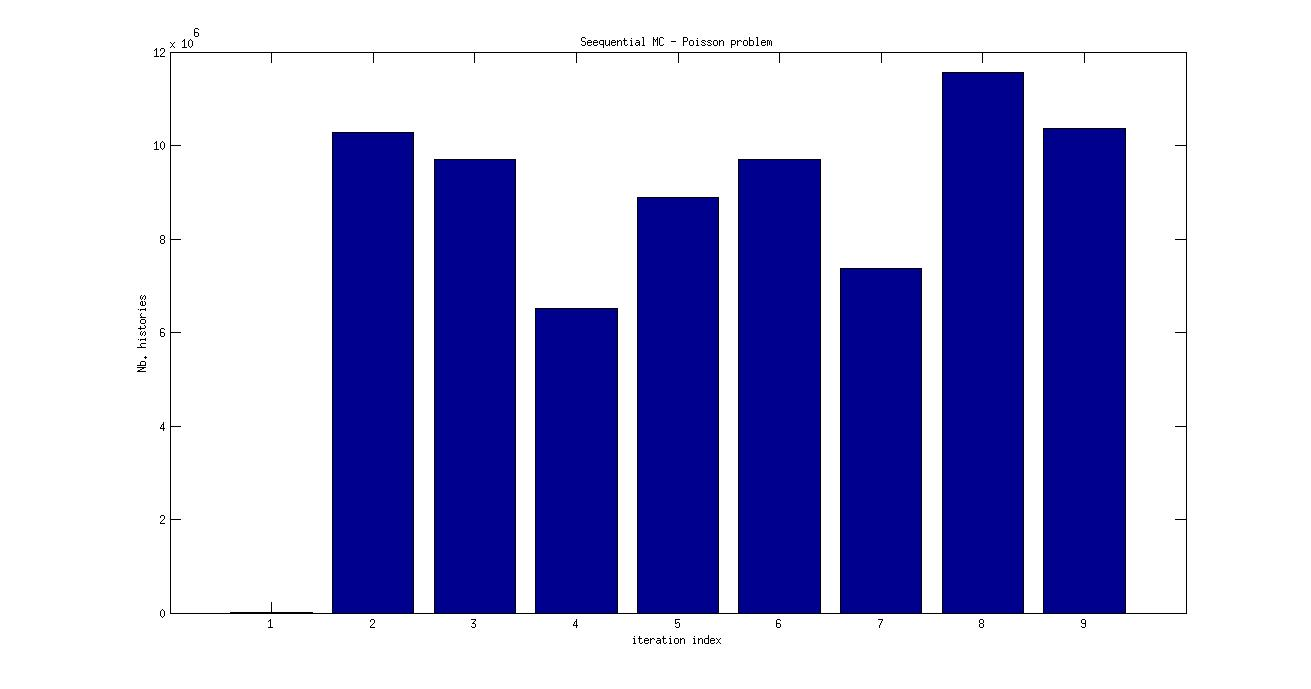
\includegraphics[width=\textwidth]{SEQ_poisson.jpg}
    \caption{Sequential MC - Poisson problem. Number of random walks employed
at each numerical iteration.}
\label{SEQ_poisson}
\end{figure}


\begin{figure}[h!]
  \centering
    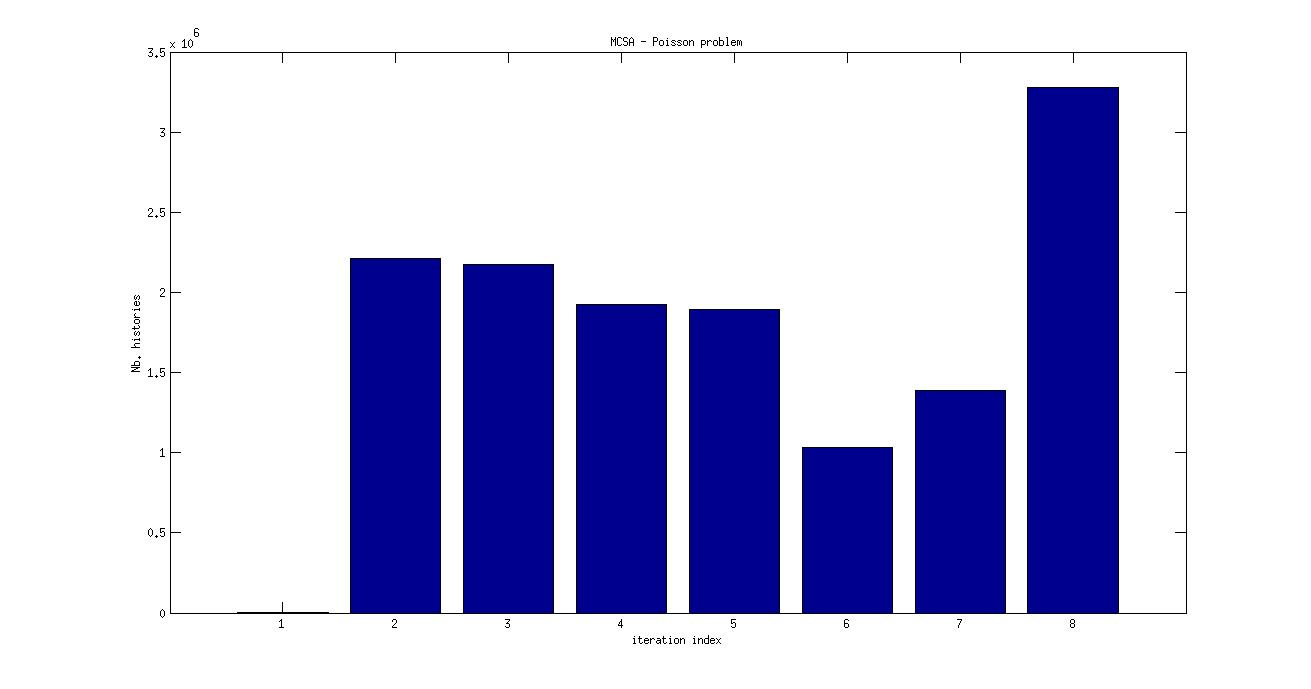
\includegraphics[width=\textwidth]{MCSA_poisson.jpg}
      \caption{MCSA - Poisson problem. Number of random walks employed at each
numerical iteration.}
\label{MCSA_poisson}
\end{figure}

\subsubsection{Reaction-Diffusion Problem}

By modifying the equation of the previous test case, we consider now
an advection reaction problem

\begin{equation}
\begin{cases}
 -\Delta u +\sigma u= f \quad \text{in}\quad \Omega \\
 u=0\quad \text{on} \quad \partial\Omega
 \end{cases}
\end{equation}
where $\Omega=(0,1)\times (0,1)$, $\sigma=0.1$ and $f=1$.
A finite difference scheme is applied to discretize the problem.
The number of nodes
on each direction of the domain is 100, so that $h\approx 0.01$. The
discretized problem has 9604 d.o.f's. A left
diagonal preconditioning is still applied to
the stiffness matrix obtained from the discretization. The 1-norm of the
iteration matrix is $\lVert H\rVert_1\approx 0.9756$. This automatically
guarantees the convergence of the Adjoint Monte Carlo linear solver. The
computation of the solution to the partial differential problem is still
accomplished with the MCSA algorithm. A threshold of $\varepsilon =10^{-8}$ is
used as a stop criterion for the relative residual. The threshold
for the adaptive selection of the random walks instead is set
to $\varepsilon_1=0.1$.
In Table \ref{DR_results} a comparison between the deterministic Synthetic
Acceleration
scheme, Sequential MC and the MCSA is provided.
The employment of the MCSA provides a significant reduction of the number of
histories necessary to satisfy the convergence criterion, in line with results
coming from the previous test case.

\begin{table}[!h]
\centering
\hspace*{-0.8cm}
\begin{tabular}{|c|c|c|c|}
\hline
algorithm & relative err.& \# iterations & average \# histories per iteration\\
\hline
 Synthetic acceleration & $9.073\cdot 10^{-8}$ & 634 & - \\
\hline
 Sequential MC & $8.415 \cdot 10^{-8}$ &  8 & 12,391,375\\
 \hline
 Adjoint MCSA & $6.633 \cdot 10^{-8}$ &  7 & 3,163,700\\
\hline
\end{tabular}
\caption{Numerical results for the diffusion reaction problem.}
\label{DR_results}
\end{table}


\begin{figure}[h!]
  \centering
    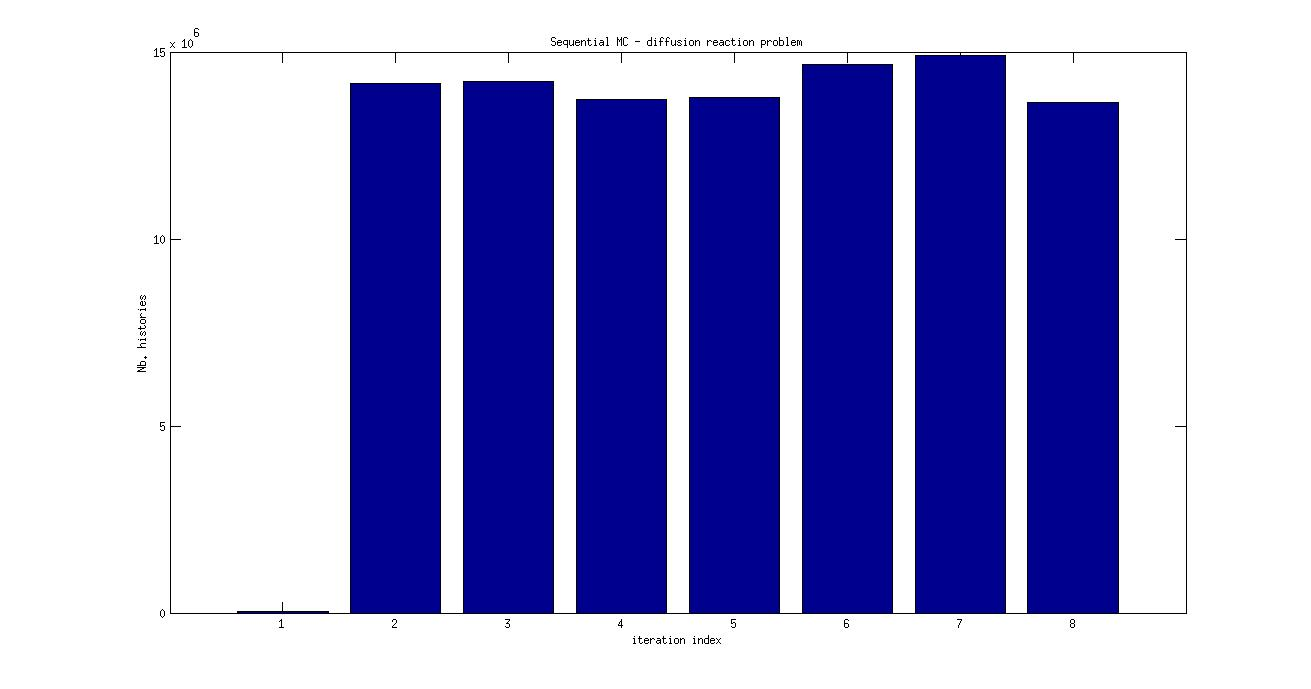
\includegraphics[width=\textwidth]{SEQ_diffreac.jpg}
      \caption{Sequential MC - Diffusion reaction problem. Number of random
walks
employed at each
numerical iteration.}
\label{SEQ_diffreac}
\end{figure}


\begin{figure}[h!]
  \centering
    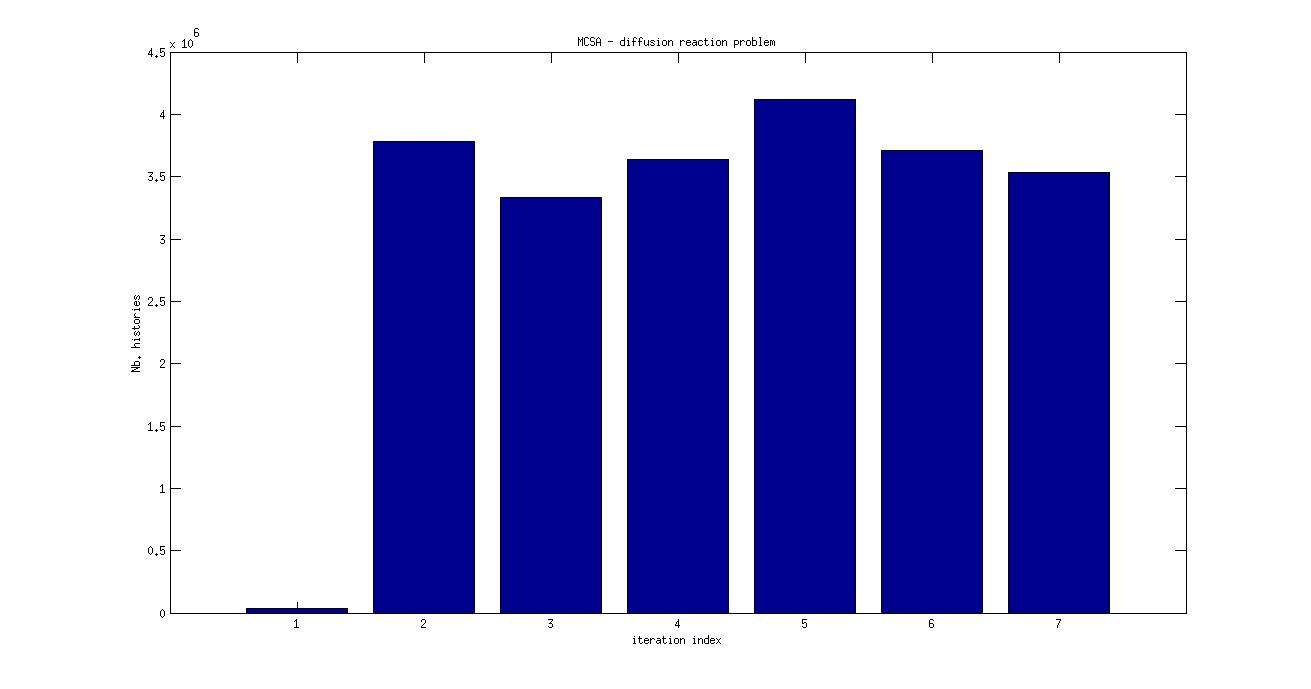
\includegraphics[width=\textwidth]{MCSA_diffreac.jpg}
      \caption{MCSA - Diffusion reaction problem. Number of random walks
employed at each
numerical iteration.}
\label{MCSA_diffreac}
\end{figure}

\subsubsection{Parabolic Problem}

In this subsection we restrict our treatise to the analysis of parabolic
partial
differential problems of the form
\begin{equation}
\begin{cases}
 \frac{\partial u }{\partial t} + \mathcal{L}(u)=f \quad \text{in} \Omega \\
\text{B.C.} \quad \text{on}\quad \delta \Omega.
\end{cases}
\label{parabolic}
\end{equation}

The partial derivative in time is discretized with finite differences, whereas
quadrilateral linear finite elements are employed for the space discretization.
Naming $N_h$ the number of d.o.f.'s associated with the finite element
discretization, the problem \ref{parabolic} turn into a fully discretized
problem such as:

\[
 \bigg (\frac{1}{\Delta t}M+A\bigg )(\mathbf{u}^{k+1}-\mathbf{u}^k)+A[\theta
\mathbf{u}^{k+1}+(1-\theta)\mathbf{u}^k]=\theta
\mathbf{f}^{k+1}+(1-\theta)\mathbf{f}^k,
\]

where $k$ is an index that goes with the time dimension.

By tuning the value of the parameter $\theta$ different numerical schemes can
be obtained with different properties of numerical stability.
However our discussion is not involved in this kind of issues.
In particular we restrict our attention to a single generic time step
associated with an Implicit Euler time discretization (corresponding to
$\theta=1$). The vector of the right hand side is chosen so that the exact
solution to the linear system for the specific time step chosen is a unit
vector $\tilde{\mathbf{u}}=\mathbbm{1}^{N_h}$.

By referring to $h$ as the space discretization step, we pick
\[
 \Delta t \le C h.
\]


Give an open and bounded set $\Omega=(0,1)\times(0,1)$, we consider the
following problem
\begin{equation}
 \begin{cases}\frac{\partial u}{\partial t} -\mu \Delta u
+\boldsymbol{\beta}(\mathbf{x})\cdot \nabla u=0, \;\; \quad \quad
\mathbf{x}\in \Omega,\quad t\in(0,T] \\
u(\mathbf{x},0) = u_0, \qquad \qquad \qquad \qquad \quad \mathbf{x}\in
\Omega \\
u(\mathbf{x},t)=u_D(\mathbf{x}),  \; \, \, \qquad \qquad \qquad \quad
\mathbf{x}\in \partial
\Omega, \quad t\in(0,T],
 \end{cases}
\end{equation}

where $\mu=\frac{3}{200}$, $\boldsymbol{\beta}(\mathbf{x})=[2y(1-x^2),\;
-2x(1-y^2)]^T$, \\$u_D=0$ on $\{\{x=0\}\times (0,1)\}$, $\{(0,1)\times
\{y=0\}\}$, $\{(0,1)\times \{y=1\}\}$.\newline

The discretization of the problem is realized with the \texttt{IFISS} toolbox.
The value of the discretization step is $h=2^{-8}$, generating a discretized
linear system with 66,049 d.o.f.'s.
As concerns the time discretization, the time step is set to $\Delta t =
10h$.\newline

The sparse approximate inverse is employed for
the linear system at hand as a right preconditioner, with a drop tolerance of
$\tau=0.05$ for both the factors.

In this situation it is not possible to
resort to any of the sufficient conditions to verify the convergence. Therefore
the only viable option is the explicit computation of the spectral radii of $H$
and $\hat{H}$.
The spectral radius of the iteration matrix is $\rho(H)\approx
0.9218$ and the spectral radius of $\hat{H}$ for the Adjoint Monte Carlo is
$\rho(\hat{H})\approx 0.9148$. The transition probability employed is the
Almost
Optimal one. Resorting to a Uniform Probability in this case would have impeded
the
convergence, since in this case $\rho(\hat{H})\approx 1.8401$.
Therefore
this is an example demonstrating that the Almost Optimal Probability
facilitates the performance of the stochastic algorithm, outperforming the
Uniform one.

The fill-in effect is
\[
 \frac{nnz(H)}{nnz(A)}=4.26,
\]
therefore the relative number of nonzero elements in $H$ is still acceptable
in terms of sparsity pattern and memory storage.

The threshold for the check on the relative residual is set to $\varepsilon
=10^{-8}$ is, whilst the threshold
for the adaptive selection of the random walks is set
to $\varepsilon_1=0.1$.
In order to test the effectiveness of employing the MCSA with respect to a
purely deterministic scheme, a comparison with the Richardson algorithm and
the Sequential Monte Carlo is
accomplished. The results are shown in Table \ref{parabolic_results}. As you
can see, the adoption of both Sequential Monte Carlo and MCSA reduces
dramatically the number of iterations with
respect to the fixed point method. Of course this
advantage has the
increase of the computational time as a payoff. Nevertheless we put off this
discussion which is of
interest for a parallelized implementation of the method. Even more the number
of random walks employed by the Sequential MC is higher than the one associated
with the MCSA, in accordance with the previous results.

\begin{table}[!h]
\centering
\hspace*{-0.8cm}
\begin{tabular}{|c|c|c|c|}
\hline
algorithm & relative err.& \# iterations & average \# histories per iteration\\
\hline
 Richardson & $6.277\cdot 10^{-7}$ & 178 & - \\
 \hline
 Sequential MC & $1.918 \cdot 10^{-9}$ & 8 & 51,535,375\\
\hline
 Adjoint MCSA & $1.341\cdot 10^{-9}$ & 6 & 16,244,000\\
\hline
\end{tabular}
\caption{Numerical results for the parabolic problem.}
\label{parabolic_results}
\end{table}


\begin{figure}[h!]
  \centering
    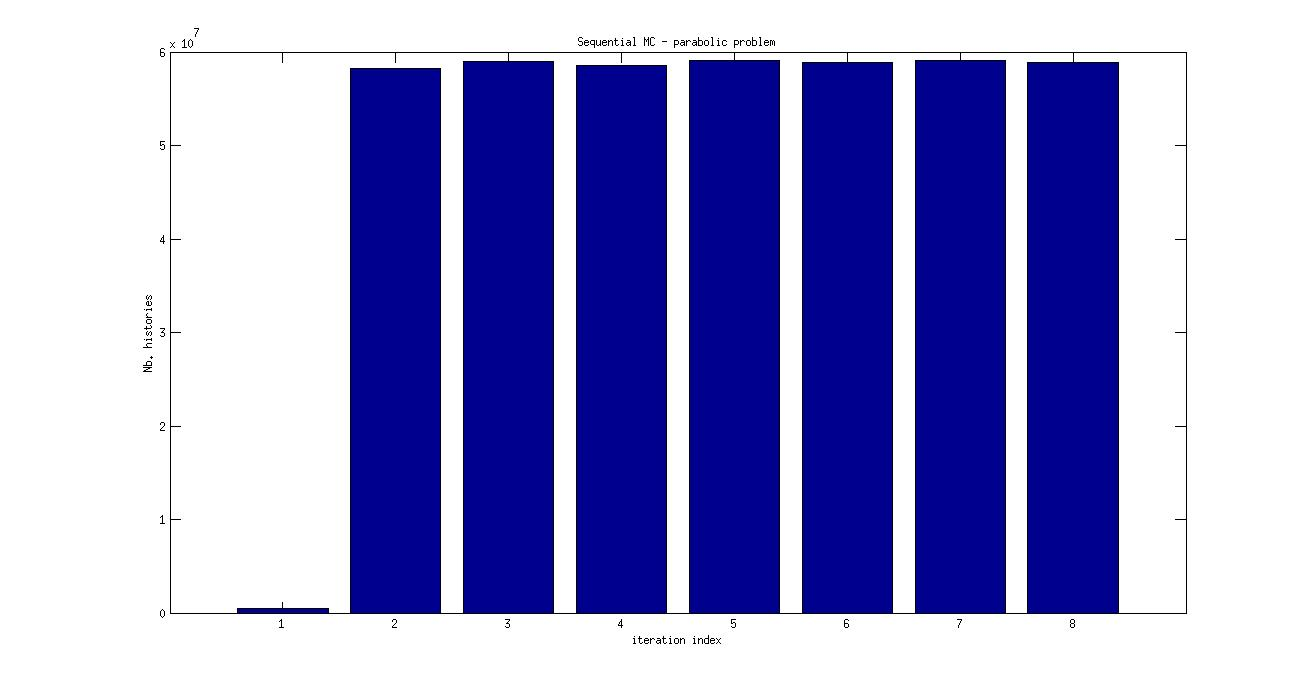
\includegraphics[width=\textwidth]{SEQ_parabolic.jpg}
      \caption{Sequential Monte Carlo - Parabolic problem. Number of random
walks
employed at each
numerical iteration.}
\label{MCSA_parabolic}
\end{figure}


\begin{figure}[h!]
  \centering
    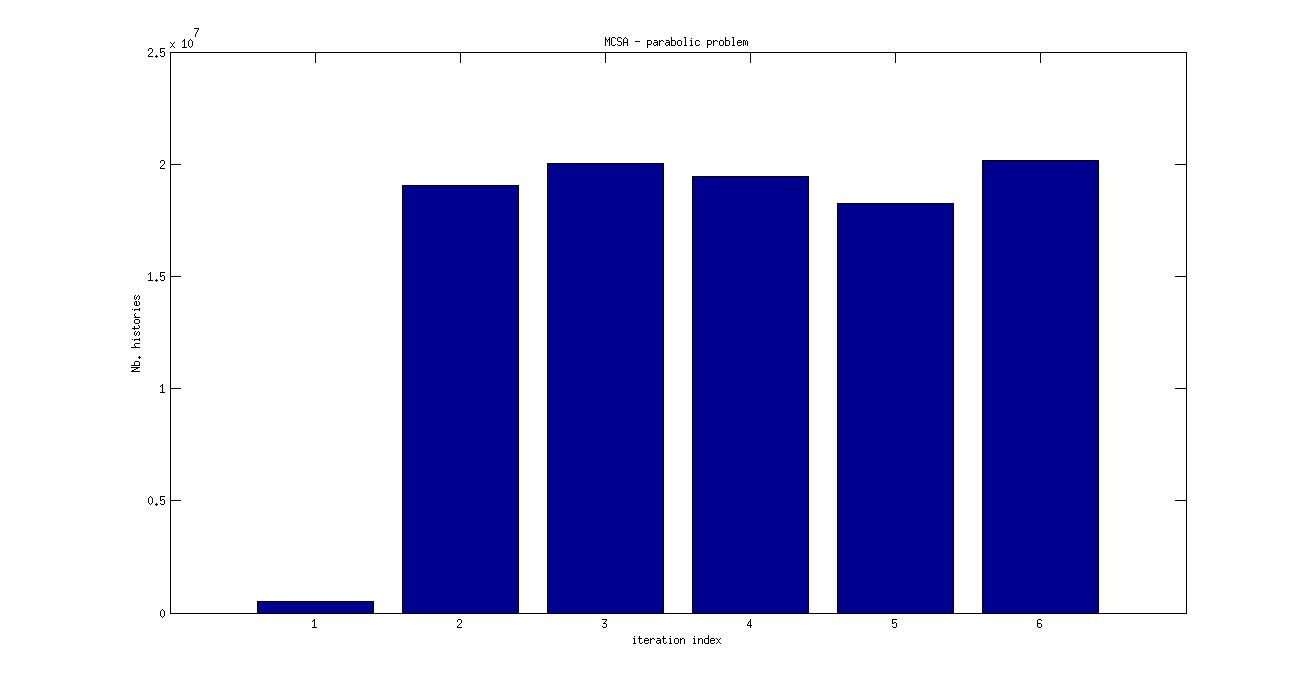
\includegraphics[width=\textwidth]{MCSA_parabolic.jpg}
      \caption{MCSA - Parabolic problem. Number of random walks
employed at each
numerical iteration.}
\label{MCSA_parabolic}
\end{figure}

